\chapter {Magnetická rezonancia}
Magnetická rezonancia (MR) je jedna zo zobrazovacích techník, ktorá je používaná k zobrazeniu vnútorných orgánov tela.
Narozdiel od röntgenového žiarenia a počítačovej tomografie (CT), magnetická rezonancia nepoužíva ionizujúce žiarenie. Avšak medzi spoločné znaky týchto troch zobrazovacích techník patrí ich neinvazívnosť a bezbolestné vyšetrenie \cite{basic_principles_of_mri} (vlastný preklad). \newline

Magnetická rezonancia sa používa najmä pri:
\begin {itemize}
\item {podozrení na anomálie mozgu a miechy, nádory a cysty,}
\item {poranení kĺbov a mäkkých tkanív,}
\item {podozrení na srdcové problémy,}
\item {rozličných ochoreniach pečene a iných brušných orgánov, atď. \cite{mr_usage} (vlastný preklad).}
\end {itemize}

Pred niektorými MR procedúrami sa pacientovi môže intravenózne podať kontrastná látka, ktorá zlepší kontrast a vzájomnú odlíšiteľnosť orgánov a mäkkých tkanív \cite{contrast_agents}.

Bohužiaľ, existujú aj určité kontraindikácie, pri ktorých použitie MR pre daného človeka nie je možné.
Jedným z kontraindikácií je implantovaný kardiostimulátor, v prípade že nie je kompatibilný s MR prístrojom. Všeobecne sa za kontraindikáciu považuje použitie akéhokoľvek magnetického materiálu v tele. Taktiež je MR vyšetrenie kontraindikované ženám v prvom trimestri tehotenstva \cite{mr_contraindications}.

\clearpage

\section {Princíp magnetickej rezonancie}
Princípom magnetickej rezonancie je smerové magnetické pole (moment - $\mathcal{B}_{0}$) spojené s pohybom voľných jadier vodíku v tele subjektu. Tieto jadrá majú charakteristický pohyb (spin) vytvárajúci malý magnetický moment s určitým smerom (ktorý je náhodný) a veľkosťou. Keď je subjekt umiestnený vo veľkom magnetickom poli (v tubuse MR prístroja), voľné vodíkové jadrá sa zarovnajú v smere $\mathcal{B}_{0}$ (smer $y$) a vytvoria magnetický moment $\mathcal{M}$ paralelne k $\mathcal{B}_{0}$. Vodíkové jadrá začnú náhle prechádzať okolo smeru magnetického poľa ako gyroskopy. Toto správanie sa nazýva Larmorova precesia \cite{basic_principles_of_mri} (vlastný preklad).

\begin {center}
        \centering
        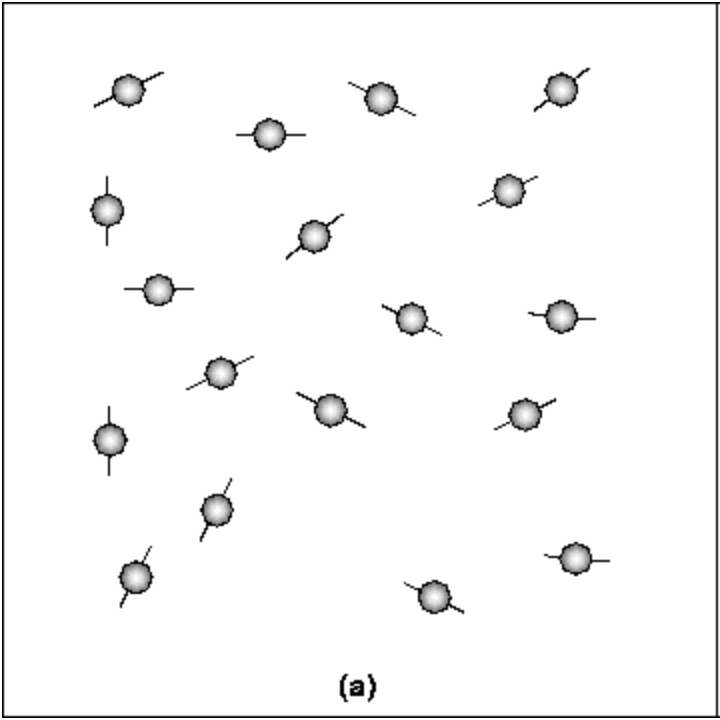
\includegraphics[width=6cm, height=6cm]{media/hydrogen/hydrogen_moving_freely.png}
        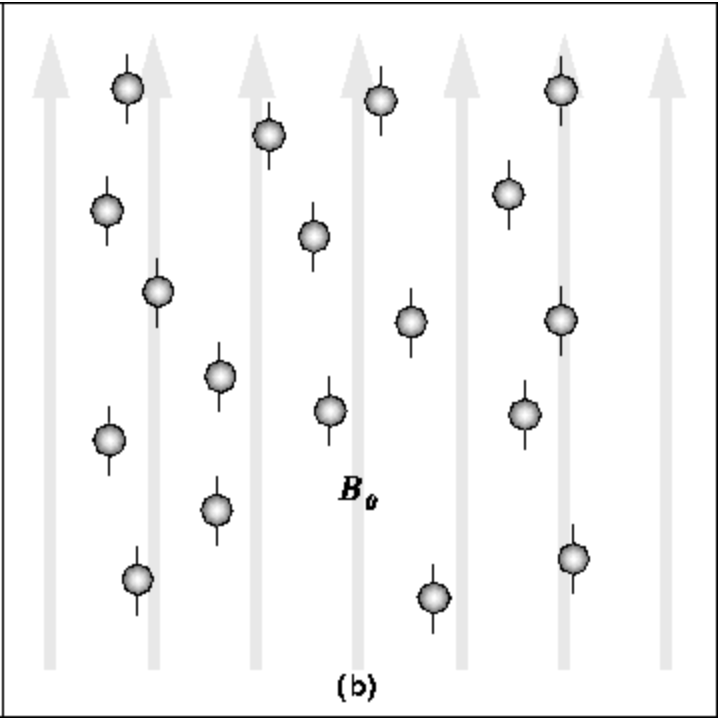
\includegraphics[width=6cm, height=6cm]{media/hydrogen/hydrogen_oscilating.png}
        \captionsetup{justification=centering}
        \captionof{figure}[Voľný pohyb vodíkových jadier a ich zarovnanie v smere $\mathcal{B}_{0}$]{Na ľavom obrázku je možné vidieť voľný pohyb vodíkových jadier a na pravom ich zarovnanie v smere $\mathcal{B}_{0}$ \cite{basic_principles_of_mri}.}
\end {center}

Následne sa aplikuje rádiofrekvenčný impulz $\mathcal{B}_{rf}$ kolmo na $\mathcal{B}_{0}$.
Tento impulz rovnajúci sa frekvencii Larmorovej precesie spôsobí posun $\mathcal{M}$ od $\mathcal{B}_{0}$ \cite{basic_principles_of_mri} (vlastný preklad).

\begin {center}
        \centering
        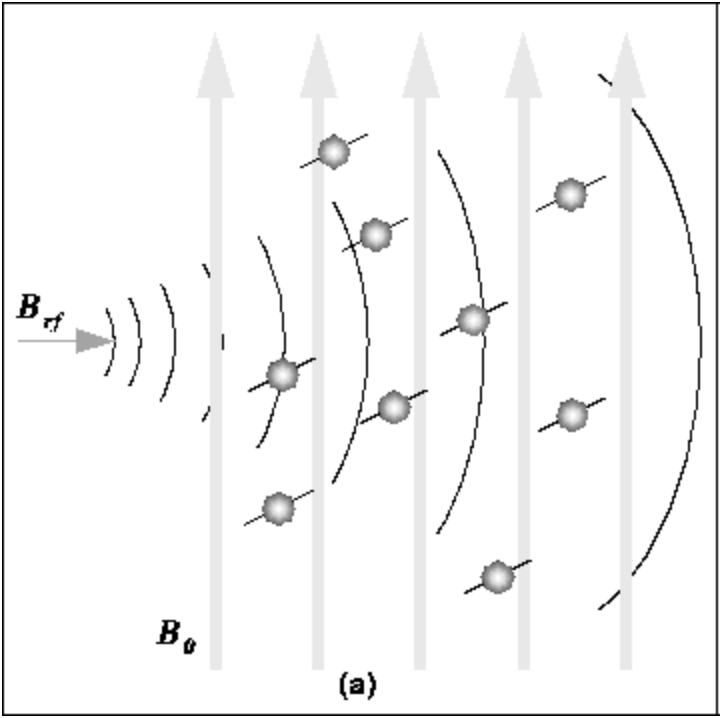
\includegraphics[width=6cm, height=6cm]{media/hydrogen/hydrogen_reacting_to_rf.png}
        \captionsetup{justification=centering}
        \captionof{figure}[Kolmá aplikácia RF impulzu $\mathcal{B}_{rf}$ na vodíkové jadrá]{Kolmá aplikácia RF impulzu $\mathcal{B}_{rf}$ na vodíkové jadrá \cite{basic_principles_of_mri}.}
\end {center}

\clearpage

Frekvenciu Larmorovej precesie (nazývaná ako Larmorova frekvencia), je definovaná nasledovne:

\begin {center}
$\omega_{0}$ = $-\gamma * \mathcal{B}_{0}$,
\end {center}

kde $\gamma$ predstavuje gyromagnetický pomer a $\mathcal{B}_{0}$ intenzitu magnetického poľa.
Gyromagnetický pomer je konštanta závislá na jadre danej častice. Pre vodík sa táto konštanta rovná 42.6 MHz/Tesla \cite{basic_principles_of_mri} (vlastný preklad). \newline

Akonáhle prestane pôsobiť rádiofrekvenčný impulz $\mathcal{B}_{rf}$, jadrá vodíka sa presunú naspäť tak, že ich $\mathcal{M}$ je znovu paralelný s $\mathcal{B}_{0}$. Tento návrat vodíkových jadier sa nazýva relaxácia. Počas nej jadrá strácajú energiu vysielaním ich vlastného rádiofrekvenčného signálu. Tento signál sa nazýva \uv{voľný indukčný rozpad} -- z anglického Free Induction Decay (FID). Ten sa zmeria vodivým poľom MR prístroja za účelom vyhotovenia 3D MR snímku v odtieňoch šedej \cite{basic_principles_of_mri} (vlastný preklad).

\begin {center}
        \centering
        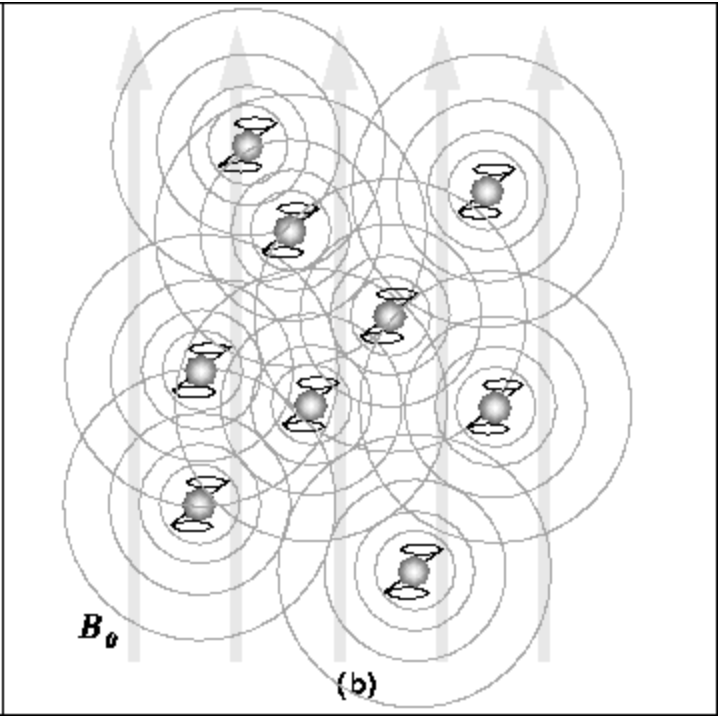
\includegraphics[width=6cm, height=6cm]{media/hydrogen/hydrogen_emitting_rf.png}
        \captionsetup{justification=centering}
        \captionof{figure}[Emitovanie FID signálu vodíkovými jadrami]{Emitovanie FID signálu vodíkovými jadrami \cite{basic_principles_of_mri}.}
\end {center}

Avšak, na jeho vytvorenie musí byť FID signál enkódovaný pre každý rozmer pomocou frekvenčného a fázového kódovania. Kódovanie v axiálnom smere sa dosiahne pridaním gradientového magnetického poľa $\mathcal{G}_{y}$ v smere $\mathcal{B}_{0}$ (v smere $y$). Po pridaní $\mathcal{G}_{y}$ sa hodnota Larmorovej frekvencie zmení lineárne v axiálnom smere, tzn. že pre konkrétny axiálny rez existuje konkrétna Larmorova frekvencia, ktorá sa aplikuje vyslaním rádiofrekvenčného impulzu $\mathcal{B}_{rf}$. $\mathcal{G}_{y}$ sa potom odstráni a ďalší gradient, $\mathcal{G}_{x}$, sa aplikuje kolmo na $\mathcal{G}_{y}$. Výsledkom je, že rezonančné frekvencie jadier sa menia v smere $x$ vďaka $\mathcal{G}_{x}$ a majú fázovú variáciu v smere $y$ v dôsledku predtým aplikovaného $\mathcal{G}_{y}$. Vzorky v smere $x$ sú teda kódované frekvenciou a v smere $y$ fázou. 2D inverzná Fourierova transformácia sa následne použije pre transformáciu vzoriek na snímku \cite{basic_principles_of_mri} (vlastný preklad). \clearpage

Kontrast získanej snímky závisí od nasledujúcich dvoch parametrov:

\begin {itemize}
\item {od času pozdĺžnej relaxácie - T1}
\item {a od času priečnej relaxácie - T2.}
\end {itemize}

Čas T1 je čas potrebný pre jadrá vodíkov k ich relaxácii a čas T2 predstavuje čas za ktorý sa FID signál prechádzajúci cez dané tkanivo rozpadne. Oba časy závisia od daného typu látky nachádzajúcej sa v subjekte \cite{basic_principles_of_mri} (vlastný preklad).

Po získaní MR snímky sa impulz $\mathcal{B}_{rf}$ opakuje vopred stanovenou rýchlosťou. Zmenou sekvencie impulzov ($\mathcal{B}_{rf}$) sa vytvárajú rôzne typy snímkov. Čas opakovania ($TR$) je množstvo času medzi po sebe nasledujúcimi pulznými sekvenciami aplikovanými na rovnaký rez. Time to Echo ($TE$) je čas medzi dodaním impulzu $\mathcal{B}_{rf}$ a prijatím odozvy. Úpravou $TR$ je možné meniť výsledný kontrast na snímke medzi rôznymi typmi tkanív \cite{basic_principles_of_mri} (vlastný preklad).

\section {SPAMM}
SPAMM -- z anglického (SPAtial Modulation of Magnetization) $\rightarrow$ \uv{priestorová modulácia magnetizácie} -- je technika používajúca rádiofrekvenčné saturačné impulzy pre umiestnenie mriežky na myokard, za cieľom sledovania jeho pohybu počas srdcového cyklu.

V súčasnej praxi sa SPAMM technika používa v situáciách, kde informácia o kontrakcii myokardu je kľúčová, ako napr. podozrenie na ischemickú chorobu srdca alebo abnormality týkajúcej sa neprirodzeného pohybu steny myokardu \cite{spamm_description} (vlastný preklad).

\begin {center}
        \centering
        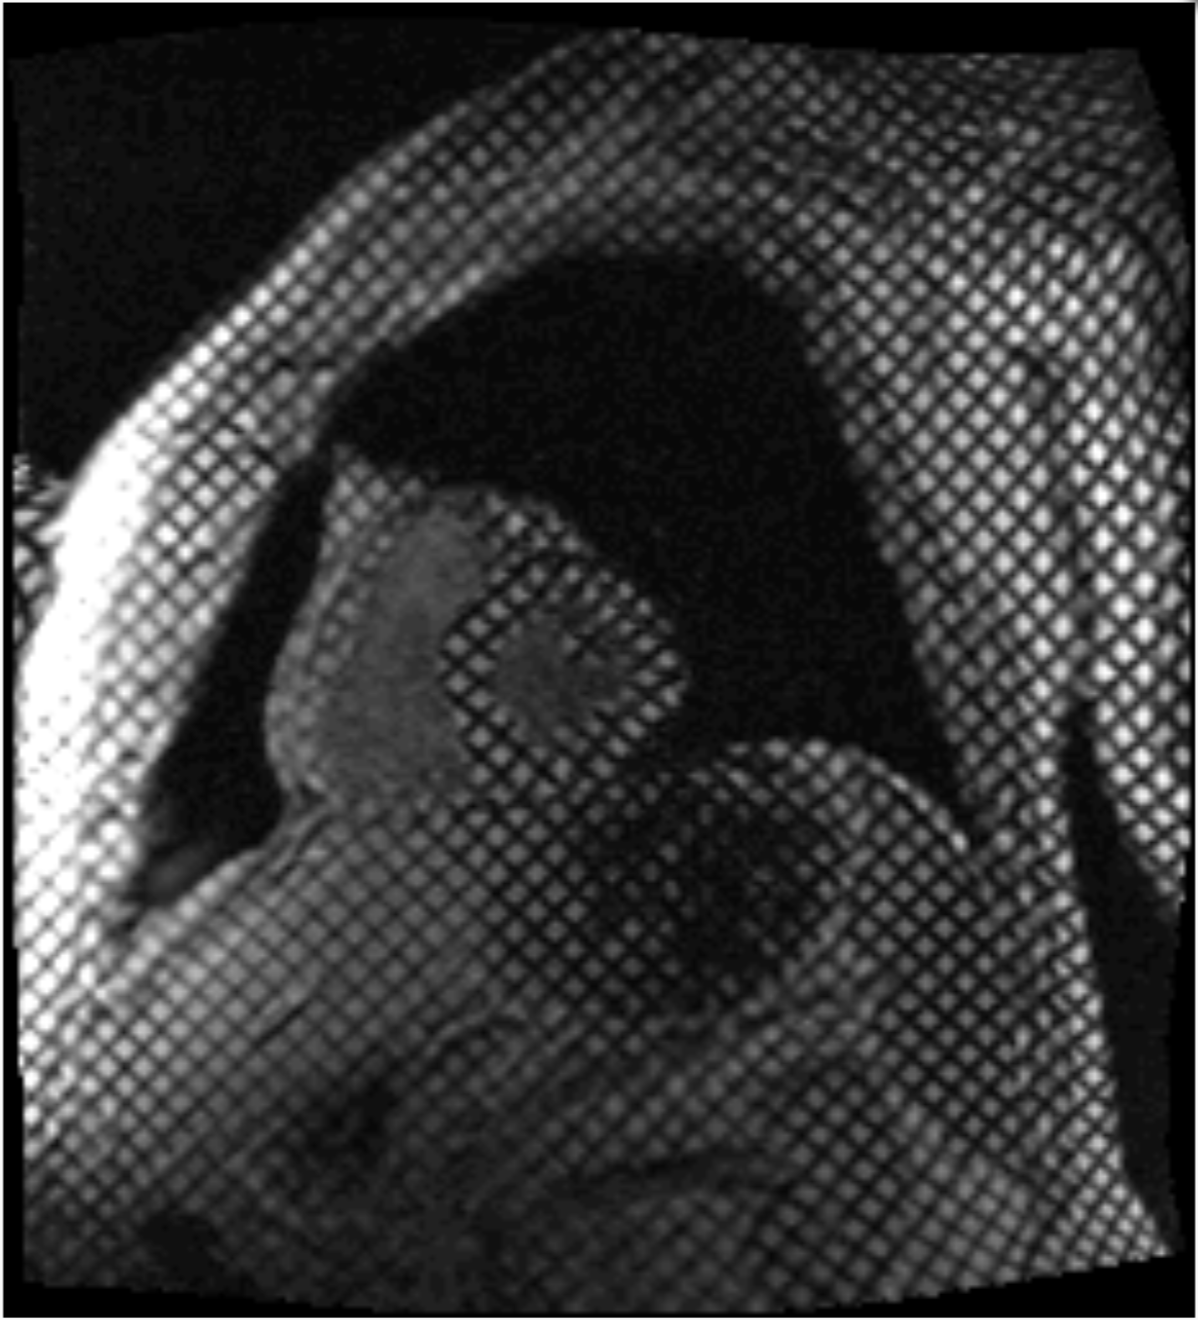
\includegraphics[width=6cm, height=6cm]{media/heart/tagged_heart.png}
        \captionsetup{justification=centering}
        \captionof{figure}[Tagovaný snímok myokardu pomocou techniky SPAMM]{Otagovaný snímok myokardu pomocou techniky SPAMM \cite{spamm_description}.}
\end {center}

\clearpage

Nevýhodou použitia tejto techniky je skutočnosť, že táto mriežka sa stráca s blížiacim sa koncom srdcového cyklu. Samotné čiary mriežky sa pri konci systoly (časť srdcového cyklu, počas ktorej sa komory srdca sťahujú po naplnení krvou) môžu zlúčiť alebo úplne vyblednúť, čo sťažuje následnú analýzu pohybu srdca \cite{spamm_description} (vlastný preklad).

\begin {center}
        \centering
        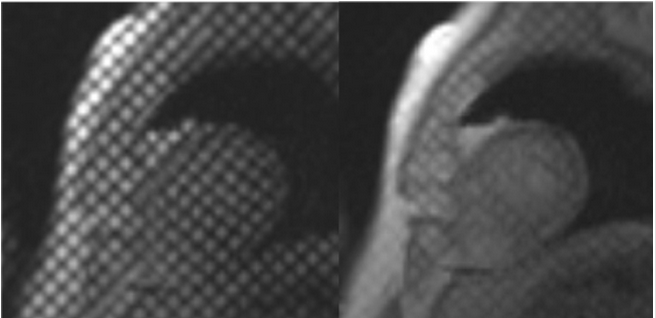
\includegraphics[width=11.5cm, height=6cm]{media/heart/early_late_systole.png}
        \captionsetup{justification=centering}
        \captionof{figure}[Ukážka vyblednutia SPAMM mriežky]{Ľavý obrázok zobrazuje začiatok systoly, pravý jej koniec.}
\end {center}